%; whizzy paragraph -pdf xpdf -latex ./whizzypdfptex.sh
%; whizzy-paragraph "^\\\\begin{frame}\\|\\\\emtext"
% latex beamer presentation.
% platex, latex-beamer $B$G%3%s%Q%$%k$9$k$3$H$rA[Dj!#(B 

%     Tokyo Debian Meeting resources
%     Copyright (C) 2012 Junichi Uekawa

%     This program is free software; you can redistribute it and/or modify
%     it under the terms of the GNU General Public License as published by
%     the Free Software Foundation; either version 2 of the License, or
%     (at your option) any later version.

%     This program is distributed in the hope that it will be useful,
%     but WITHOUT ANY WARRANTY; without even the implied warreanty of
%     MERCHANTABILITY or FITNESS FOR A PARTICULAR PURPOSE.  See the
%     GNU General Public License for more details.
%     You should have received a copy of the GNU General Public License
%     along with this program; if not, write to the Free Software
%     Foundation, Inc., 51 Franklin St, Fifth Floor, Boston, MA  02110-1301 USA

\documentclass[cjk,dvipdfmx,12pt]{beamer}
\usetheme{Tokyo}
\usepackage{monthlypresentation}

%  preview (shell-command (concat "evince " (replace-regexp-in-string "tex$" "pdf"(buffer-file-name)) "&")) 
%  presentation (shell-command (concat "xpdf -fullscreen " (replace-regexp-in-string "tex$" "pdf"(buffer-file-name)) "&"))
%  presentation (shell-command (concat "evince " (replace-regexp-in-string "tex$" "pdf"(buffer-file-name)) "&"))

%http://www.naney.org/diki/dk/hyperref.html
%$BF|K\8l(BEUC$B7O4D6-$N;~(B
\AtBeginDvi{\special{pdf:tounicode EUC-UCS2}}
%$B%7%U%H(BJIS$B7O4D6-$N;~(B
%\AtBeginDvi{\special{pdf:tounicode 90ms-RKSJ-UCS2}}

\newenvironment{commandlinesmall}%
{\VerbatimEnvironment
  \begin{Sbox}\begin{minipage}{1.0\hsize}\begin{fontsize}{8}{8} \begin{BVerbatim}}%
{\end{BVerbatim}\end{fontsize}\end{minipage}\end{Sbox}
  \setlength{\fboxsep}{8pt}
% start on a new paragraph

\vspace{6pt}% skip before
\fcolorbox{dancerdarkblue}{dancerlightblue}{\TheSbox}

\vspace{6pt}% skip after
}
%end of commandlinesmall

\title{$BEl5~%(%j%"(BDebian$BJY6/2q(B}
\subtitle{$BBh(B143$B2s(B 2016$BG/(B9$B7nEY(B}
\author{$B?yK\(B $BE5=<(B}
\date{2016$BG/(B9$B7n(B17$BF|(B}
\logo{
\includegraphics[width=8cm]{image200607/openlogo-light.eps}}

\begin{document}

\begin{frame}
\titlepage{}
\end{frame}

\begin{frame}{Agenda}
 \begin{minipage}[t]{0.45\hsize}
  \begin{itemize}
  \item $B:G6a$"$C$?(BDebian$B4XO"$N%$%Y%s%HJs9p(B
	\begin{itemize}
	\item $BBh(B142$B2sEl5~%(%j%"(BDebian$BJY6/2q(B
	\end{itemize}
  %\item $B;vA02]BjH/I=(B
  \end{itemize}
 \end{minipage}
 \begin{minipage}[t]{0.45\hsize}
  \begin{itemize}
   \item Debian Trivia Quiz
  \end{itemize}
 \end{minipage}
\end{frame}

\section{$B%$%Y%s%HJs9p(B}
\emtext{$B%$%Y%s%HJs9p(B}

\begin{frame}{$BBh(B142$B2sEl5~%(%j%"(BDebian$BJY6/2q(B}

\begin{itemize}
\item $B>l=j$OD+F|%M%C%H$5$s$r$*<Z$j$7$F3+:E$7$^$7$?(B
\item $B;22C<T$O(B6$BL>(B
\item $B%;%_%JFbMF$O!"0J2<FbMF$rH/I=$7$^$7$?(B
  \begin{enumerate}
  \item $B?yK\$5$s!V(BDebian$B$G(Blxc$B$r%;%C%H%"%C%W$7$F$_$h$&!W(B
  \item khibino$B$5$s!V(Bhaskell-relational-record$B!W$N>R2p!JHt$S9~$_!K(B
  \end{enumerate}
\item $B;D$j$N;~4V$G(Bhack time$B$r9T$$!"@.2LH/I=$r$7$^$7$?(B
\item \url{https://tokyodebianmeeting.titanpad.com/ep/pad/export/142/rev.487?format=txt}
\end{itemize} 
\end{frame}

%\section{$B;vA02]Bj(B}
%\emtext{$B;vA02]Bj(B}
%{\footnotesize
% \begin{prework}{ 山下康成 }
  \begin{enumerate}
  \item 本日のHackTime作業
  \end{enumerate}
\end{prework}

\begin{prework}{ dictoss }
  \begin{enumerate}
  \item 本日のHackTime作業
  \end{enumerate}
\end{prework}

\begin{prework}{ NOKUBI Takatsugu }
  \begin{enumerate}
  \item 本日のHackTime作業
  \end{enumerate}
\end{prework}

\begin{prework}{ issei }
  \begin{enumerate}
  \item 本日のHackTime作業
  \end{enumerate}
\end{prework}

\begin{prework}{ iwamatsu }
  \begin{enumerate}
  \item 本日のHackTime作業
  \end{enumerate}
\end{prework}

\begin{prework}{ yy\_y\_ja\_jp }
  \begin{enumerate}
  \item 本日のHackTime作業
  \end{enumerate}
\end{prework}

\begin{prework}{ yosuke\_san }
  \begin{enumerate}
  \item 本日のHackTime作業
  \end{enumerate}
\end{prework}

%}

\subsection{$BLdBj(B}

%; whizzy-master ../debianmeetingresume201311.tex
% $B0J>e$N@_Dj$r$7$F$$$k$?$a!"$3$N%U%!%$%k$G(B M-x whizzytex $B$9$k$H!"(Bwhizzytex$B$,MxMQ$G$-$^$9!#(B
%

\santaku
{debain$B%Q%C%1!<%8$N%=!<%9%3!<%I$r%@%&%s%m!<%I$9$kJ}K!$O$"$k$+<ALd$,$"$j$^$7$?!#(BDD$B$NJ}$?$A$,0FFb$7$?%5!<%S%9$O$I$l$G$7$g$&$+!#(B}
{srcs.debian.org}
{srcs.debian.net}
{sources.debian.net}
{C}
{$B4Z9q$G>pJs9)3X$r3X$s$G$$$kBg3X1!@8$NJ}$+$i%;%-%e%j%F%#$N8&5f$N0l4D$GA4%=!<%9%3!<%I$,$[$7$$$H$N$3$H$G$7$?!#$=$N$[$+$K(Bdebmirror$B%3%^%s%I$r;H$&$H$h$$$H$$$&%"%I%P%$%9$b$"$j$^$7$?!#>pJs85(B:\url{https://lists.debian.org/debian-devel/2016/09/msg00118.html}}


\section{DEP5 Machine-readable debian/copyright $B:F9M(B}
\emtext{DEP5 Machine-readable debian/copyright $B:F9M(B}

\begin{frame}{$B$O$8$a$K(B}

\begin{itemize}
\item  Debian $B%=!<%9%Q%C%1!<%8$K$O(B debian/copyright $B%U%!%$%k$,$"$j!"$3$N%U%!%$%k$K$O(B
$BBP>]%=%U%H%&%'%"$N%i%$%;%s%9!"%3%T!<%i%$%H$,=q$+$l$F$$$k!#(B
\item 2009$BG/0JA0$OFC$K%U%)!<%^%C%H$b$J$/!"%i%$%;%s%9$bJq3gE*$J=q$-J}!#(B
\end{itemize}
\end{frame}

\begin{frame}[containsverbatim]{$B$O$8$a$K(B}
\begin{commandlinesmall}
gcc-defaults is Copyright (C) 2000, 2001, 2006, 2009 Debian.

These scripts are free software; you can redistribute it and/or modify it
under the terms of the GNU General Public License as published by the
Free Software Foundation; either version 2, or (at your option) any
later version.

On Debian GNU/Linux systems, the complete text of the GNU General
Public License can be found in `/usr/share/common-licenses/GPL'.

The c89 and c99 man pages are taken from netbsd:

Copyright (c) 1999 The NetBSD Foundation, Inc.
All rights reserved.
($B>JN,(B)
\end{commandlinesmall}
\end{frame}

\begin{frame}{$B$O$8$a$K(B}
\begin{itemize}
\item $B5!3#=hM}$G$-$k%U%)!<%^%C%H$K@Z$jBX$(!"<+F0%A%'%C%/$J$I$,$G$-$k$h$&$K$9$k$?$a!"(B
DEP5 / Machine-readable debian/copyright $B!J0J2<!"(BDEP5$B!K$,:vDj!#(B
\item $B:vDj8e(B BTS 609160 $B$K$h$C$F(B Debian Policy $B$K<h$j9~$^$l!"(BDebian Policy $B$N0l(B
$BIt$H$J$k!#(B
(Debian Policy 12.5$B!"%*%W%7%g%J%k07$$(B)
\item $B:G?7%P!<%8%g%s$O(B 1.0 $B$G$"$j!":G?7HG$O(B
\url{https://www.debian.org/doc/packaging-manuals/copyright-format/1.0/}
\end{itemize}
\end{frame}

\begin{frame}{$B$O$8$a$K(B}
\begin{itemize}
\item $BB?$/$N%Q%C%1!<%8$,(BDEP5 $B=`5r$N(B debian/copyright $B$K@Z$jBX$o$C$F$$$k!#(B
\item $BFbMF$,JQ99$5$l$:$=$N$^$^B3$1$k$H$$$&LdBj$,$"$k!#(B
\item $B:#2s$O(B DEP5 $B$K$D$$$F$N%U%)!<%^%C%H$N>R2p$H!"(Bdebian/copyright $B%U%!%$%k$N99?7J}K!$K$D$$$F(B
$B>R2p!#(B
\end{itemize}
\end{frame}


\begin{frame}{DEP5 $B%U%)!<%^%C%H$K$D$$$F(B}

\begin{itemize}
\item DEP5$B$N%U%)!<%^%C%H(B
\begin{itemize}
\item $B%X%C%@!<It(B \\
  $B%=%U%H%&%'%"A4BN$K4X$o$k>pJs!"Nc$($PHRI[85$dO"Mm@h$r5-=R(B
\item $B%U%!%$%kIt(B \\
  $B%U%!%$%kKh$N%3%T!<%i%$%H$H%i%$%;%s%9$r5-=R(B
\end{itemize}
\end{itemize}
\end{frame}

\begin{frame}{DEP5 $B%U%)!<%^%C%H$K$D$$$F(B}
$B%X%C%@!<It$GMxMQ$G$-$k%U%#!<%k%I(B
\begin{itemize}
  \item Format:
  \item Upstream-Name:
  \item Upstream-Contact:
  \item Source:
  \item Disclaimer:
  \item Comment:
  \item License:
  \item Copyright:
\end{itemize}
\end{frame}

\begin{frame}{DEP5 $B%U%)!<%^%C%H$K$D$$$F(B}
$B%U%!%$%kIt$GMxMQ$G$-$k%U%#!<%k%I(B
\begin{itemize}
  \item  Files:
  \item  Copyright:
  \item  License:
  \item  Comment:
\end{itemize}
\end{frame}

\begin{frame}[containsverbatim]{DEP5 $B%U%)!<%^%C%H$K$D$$$F(B}
\begin{commandlinesmall}
Files: *
Copyright: foo bar <foo@example.org>
License: GPL-2+

File: debian/*
Copyright: Nobuhiro Iwamatsu <iwamatsu@debian.org>
License: GPL-2+
 This program is free software; you can redistribute it
 and/or modify it under the terms of the GNU General Public
 License as published by the Free Software Foundation; either
 version 2 of the License, or (at your option) any later
 version.
 .
 This program is distributed in the hope that it will be
 useful, but WITHOUT ANY WARRANTY; without even the implied
 warranty of MERCHANTABILITY or FITNESS FOR A PARTICULAR
 PURPOSE.  See the GNU General Public License for more
 details.
 .
 You should have received a copy of the GNU General Public
 License along with this package; if not, write to the Free
 Software Foundation, Inc., 51 Franklin St, Fifth Floor,
 Boston, MA  02110-1301 USA
 .
 On Debian systems, the full text of the GNU General Public
 License version 2 can be found in the file
 `/usr/share/common-licenses/GPL-2'.
\end{commandlinesmall}
\end{frame}

\begin{frame}[containsverbatim]{DEP5 $B%U%)!<%^%C%H$K$D$$$F(B}

$B$=$NB>!"5<;w%U%#!<%k%I(B

\begin{itemize}
\item License-Grant \\
	\debianbug{786450} $B;2>H(B
\item License-Reference \\
	\debianbug{786450} $B;2>H(B
\item Files-Excluded: \\
	\debianbug{685506} $B;2>H(B
\end{itemize}
\end{frame}


\begin{frame}[containsverbatim]{DEP5 $B%U%)!<%^%C%H$K$D$$$F(B}

erlang-cowboy $B%Q%C%1!<%8$N(B debian/copyright:
\begin{commandlinesmall}
Formats: https://www.debian.org/doc/packaging-manuals/copyright-format/1.0/
upstream-name: cowboy
upstream-contact: Loc Hoguin <essen@ninenines.eu>
Source: https://github.com/extend/cowboy.git
Files-Excluded: examples/websocket/priv/static/jquery.min.js
 examples/markdown_middleware/priv/small.mp4
 examples/markdown_middleware/priv/small.ogv
 examples/static_world/priv/small.mp4
 examples/static_world/priv/small.ogv
 examples/web_server/priv/small.mp4
 examples/web_server/priv/small.ogv

Files: *
Copyright: 2011-2012, Loc Hoguin <essen@ninenines.eu>
License: ISC

Files: debian/*
Copyright: Copyright 2012, Nobuhiro Iwamatsu <iwamatsu@debian.org>
License: Apache-2.0

License: ISC
 Permission to use, copy, modify, and/or distribute this software for any
 purpose with or without fee is hereby granted, provided that the above
 copyright notice and this permission notice appear in all copies.
 .
 THE SOFTWARE IS PROVIDED "AS IS" AND THE AUTHOR DISCLAIMS ALL WARRANTIES
 WITH REGARD TO THIS SOFTWARE INCLUDING ALL IMPLIED WARRANTIES OF
 MERCHANTABILITY AND FITNESS. IN NO EVENT SHALL THE AUTHOR BE LIABLE FOR
 ANY SPECIAL, DIRECT, INDIRECT, OR CONSEQUENTIAL DAMAGES OR ANY DAMAGES
 WHATSOEVER RESULTING FROM LOSS OF USE, DATA OR PROFITS, WHETHER IN AN
 ACTION OF CONTRACT, NEGLIGENCE OR OTHER TORTIOUS ACTION, ARISING OUT OF
 OR IN CONNECTION WITH THE USE OR PERFORMANCE OF THIS SOFTWARE.

License: Apache-2.0
 On Debian systems, the full text of the Apache License (Version 2.0)
 can be found in the file  `/usr/share/common-licenses/Apache-2.0' file.

\end{commandlinesmall}
\end{frame}

\begin{frame}{DEP5 $B$NLdBjE@$HBP:v(B}

\begin{itemize}
\item DEP5 $B$O(B $B%]%j%7!<$N0lIt$G$"$k$,!"%*%W%7%g%J%k(B
\item $B0lEY:n$C$?$i$"$^$j99?7$7$J$$!#(B
\item $B5!3#E*$K%A%'%C%/!"%"%C%W!<%G!<%H$G$-$k;EAH$_$,I,MW!#(B
\end{itemize}
\end{frame}

\begin{frame}[containsverbatim]{licensecheck $B$r;H$C$?(BDEP5 $B%U%)!<%^%C%H2=(B}

licensecheck $B$K$h$k(B $B%i%$%;%s%9$H%3%T!<%i%$%H%[%k%@!<$N=PNO(B

\begin{commandline}
$ licensecheck -r --copyright .
ell/io.h: LGPL (v2.1 or later)
  [Copyright: 2011-2014 Intel Corporation. All rights reserved]

ell/dbus.c: LGPL (v2.1 or later)
  [Copyright: 2011-2014 Intel Corporation. All rights reserved]
($B>JN,(B)
\end{commandline}

\end{frame}

\begin{frame}[containsverbatim]{licensecheck $B$r;H$C$?(BDEP5 $B%U%)!<%^%C%H2=(B}

/usr/lib/cdbs/licensecheck2dep5 $B$r;H$C$?(BDEP5$B%U%)!<%^%C%H$X$N@07A(B

\begin{commandlinesmall}
$ licensecheck -r --copyright .  | /usr/lib/cdbs/licensecheck2dep5

Format: http://www.debian.org/doc/packaging-manuals/copyright-format/1.0/
Upstream-Name: FIXME
Upstream-Contact: FIXME
Source: FIXME
Disclaimer: Autogenerated by CDBS

Files: ./ell/base64.c
 ./ell/base64.h
 ./ell/checksum.c
 $B!JCfN,!K(B 
 ./unit/test-uuid.c
Copyright: 2011-2014, Intel Corporation.
  2011-2015, Intel Corporation.
  2011-2016, Intel Corporation.
  2015, Intel Corporation.
  2016, Intel Corporation.
License: LGPL (v2.1 or later)
 FIXME
$B!J>JN,!K(B 
\end{commandlinesmall}

\end{frame}

%DEP5$B%U%)!<%^%C%H$K$7$F=PNO$7$F$/$l$^$9$,!"(BLicense $B%U%#!<%k%I$,(B\texttt{FIXME}
%$B$K$J$C$F$$$?$j!"(BASCII $B0J30$NJ8;z$OJ8;z2=$1$9$k$J$I!"40`z$J=PNO$O$7$F$/$l$J$$$?$a!"(B
%$B@8@.$5$l$?%F%-%9%H$r=$@5$9$kI,MW$,$"$j$^$9!#(B

\begin{frame}[containsverbatim]{cme $B$r;H$C$?(B DEP5 $B%U%)!<%^%C%H2=$H(B debian/copyright $B$N99?7(B}

cme $B$H(B libconfig-model-dpkg-perl $B$r;H$C$?(BDEP5 $B%U%)!<%^%C%H2=(B

\begin{commandlinesmall}
$ sudo apt-get install cme libconfig-model-dpkg-perl
$ cme update dpkg-copyright
cme: using Dpkg::Copyright model
updating data
$B!J>JN,!K(B
\end{commandlinesmall}

\end{frame}


\begin{frame}[containsverbatim]{cme $B$r;H$C$?(B DEP5 $B%U%)!<%^%C%H2=$H(B debian/copyright $B$N99?7(B}
c
me$B!"(Blibconfig-model-dpkg-perl$B!"(Blibconfig-model-tkui-perl $B%Q%C%1!<%8$K$h$k(B GUI $BJT=8(B

\begin{commandlinesmall}
$ sudo apt-get install libconfig-model-tkui-perl
debian/copyright $B$rJT=8$7$?$$>l9g(B
$ cme edit dpkg-copyright
debian/copyright $B$r99?7$7$?8e!"JT=8$7$?$$>l9g(B
$ cme update dpkg-copyright --edit
$B%(%G%#%?$GD>@\JT=8$G$bBg>fIW$G$9!#(B
$ cme update dpkg-copyright
$ vi debian/copyright
\end{commandlinesmall}
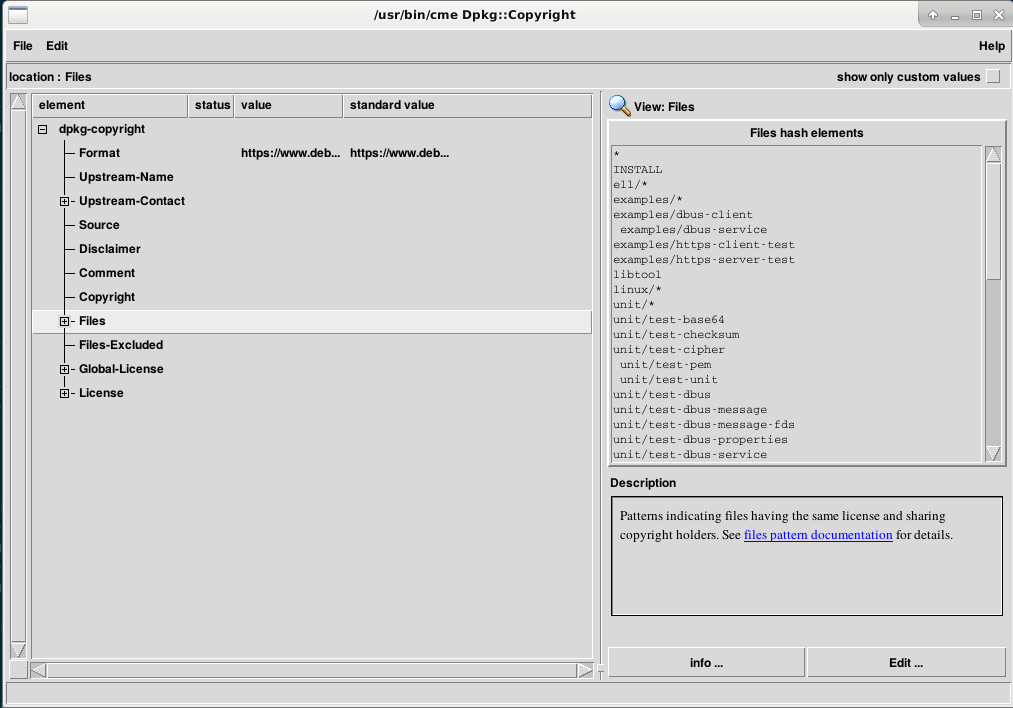
\includegraphics[width=0.7\hsize]{image201609/cme-gui.png}

\end{frame}

\begin{frame}[containsverbatim]{debmake $B$r;H$C$?(B debian/copyright $B$N(B DEP5$B%U%)!<%^%C%H2=(B}

debmake $B%3%^%s%I$N(B \texttt{-cc} $B%*%W%7%g%s$r;H$C$?(BDEP5$B%U%)!<%^%C%H2=(B

\begin{commandlinesmall}
$ debmake -cc > debian/copyright
\end{commandlinesmall}

\end{frame}

\begin{frame}[containsverbatim]{license-reconcile $B$K$h$k(B debian/copyright $B%A%'%C%/%5%]!<%H(B}

license-reconcile $B$G(B debian/copyright $BFb$N%A%'%C%/(B

\end{frame}

\begin{frame}[containsverbatim]{license-reconcile $B$K$h$k(B debian/copyright $B%A%'%C%/%5%]!<%H(B}

debian/copyright $BNc(B:
\begin{center}
\begin{commandline}
Files: *
Copyright: 2016 foo bar <foo@example.org>
License: GPL-3+
\end{commandline}
\end{center}

debian/license-reconcile.yml $BNc(B:
\begin{commandline}
Rules:
 rules:
  -
   Glob: hoge.png
   License: GPL-2+
   Copyright: 2016 foo bar <foo@example.org>
\end{commandline}

\end{frame}

\begin{frame}[containsverbatim]{license-reconcile $B$K$h$k(B debian/copyright $B%A%'%C%/%5%]!<%H(B}

license-reconcile $B<B9TNc(B:

\begin{commandline}
$ license-reconcile
License mismatch: File hoge.png has license GPL-2+ which does not match GPL-3+.\
at /usr/share/perl5/Debian/LicenseReconcile/App.pm line 222, <GEN0> line 3.
\end{commandline}

\begin{commandline}
Files: hoge.png
Copyright: foo bar <foo@example.org>
License: GPL-2+
 This program is free software: you can redistribute it and/or modify
 it under the terms of the GNU General Public License as published by
 the Free Software Foundation, either version 2 of the License, or
 (at your option) any later version.
$B!J>JN,!K(B
\end{commandline}

\end{frame}

\begin{frame}[containsverbatim]{debian $B%Q%C%1!<%8B&$NBP1~(B}

debian/rules $B$K%i%$%;%s%9%A%'%C%/MQ$N%?!<%2%C%HDI2C$K$h$kBP1~$,$*4+$a!#(B
\\
cme $B$r;H$&>l9g(B:
\begin{commandlinesmall}
update-debian-copyright:
	cme update dpkg-copyright -file debian/copyright.auto
\end{commandlinesmall}

licensecheck + licensecheck2dep5 $B$r;H$&>l9g(B:
\begin{commandlinesmall}
update-debian-copyright:
        licensecheck --copyright -r `find * -type f` | \
                /usr/lib/cdbs/licensecheck2dep5 > debian/copyright.auto
\end{commandlinesmall}
\end{frame}

\begin{frame}{$B$^$H$a(B}

\begin{itemize}
\item DEP 5 $B$O(B Debian $B%]%j%7!<$N0lIt!#$7$+$7%*%W%7%g%J%k07$$!#(B
\item licensecheck $B%D!<%k$K$h$C$F(B $B%=!<%9$+$i$N%i%$%;%s%9$H%3%T!<%i%$%H%[%k%@!<$r(B
$BCj=P2DG=!#$=$N$^$^$G$O(BDEP5$B%U%)!<%^%C%H$K$J$i$J$$$?$a!"(Blicensecheck2dep5$B$r;H$&!#(B
\item cme $B$H(B libconfig-model-dpkg-perl $B$r;H$&$3$H$K$h$C$F(B licensecheck +
licensecheck2dep5 $BF1MM$N$3$H$,2DG=!#4d>>$N$*4+$a$O$3$A$i!#(B
\item license-reconcile $B$r;H$&$3$H$K$h$C$F(B cme $B$J$I$GJd40$G$-$J$$%U%!%$%k$N%A%'(B
$B%C%/$,$G$-$k!#(B
\item $BKh2s(B cme $B$d(B licencecheck $B$J$I$N%3%^%s%I$r<B9T$9$k$N$G$O$J$/!"(Bdebian/rules 
$B$K=q$$$F$*$/$H%a%s%F%J%s%9$,3Z$K$J$k!#(B
\end{itemize}

\end{frame}

\section{Hack time}
\emtext{Hack time}

\begin{frame}{$B@.2L$r5-F~2<$5$$(B!}

  $B:#2s!"(BHack time$B;~$N@.2L$r5-O?$K;D$7$F$_$^$9!#(B

\url{https://tokyodebianmeeting.titanpad.com/143}

$B$K3'$5$s%"%/%;%9D:$-!JG'>ZITMW$G$9!K!"3F<+@.2L$r(B17:30$B$^$G$K5-O?$9$k$h$&$K$*4j$$$7$^$9!#(B

\end{frame}
  
\section{$B:#8e$N%$%Y%s%H(B}
\emtext{$B:#8e$N%$%Y%s%H(B}
\begin{frame}{$B:#8e$N%$%Y%s%H(B}
\begin{itemize}
\item 10/15($BEZ(B) $BEl5~%(%j%"(BDebian$BJY6/2q(B($BM=Dj(B)
  \begin{itemize}
  \item $BH/I=<TJg=8Cf(B
  \end{itemize}
\item 11/5($BEZ(B),6($BF|(B) OSC 2016 Tokyo/Spring
  \begin{itemize}
  \item $B%;%_%J!<$O(B11/5
  \item $BE8<($O(B11/5$B$,K\HV(B,11/6$B$O%A%i%7$N$_(B
  \end{itemize}
\item 11/19($BEZ(B) $BEl5~%(%j%"(BDebian$BJY6/2q(B($BM=Dj(B)
\end{itemize}
\end{frame}

\end{document}

;;; Local Variables: ***
;;; outline-regexp: "\\([ 	]*\\\\\\(documentstyle\\|documentclass\\|emtext\\|section\\|begin{frame}\\)\\*?[ 	]*[[{]\\|[]+\\)" ***
;;; End: ***
